\section{Blockchain}
In diesem Kapitel wird auf die revolutionären Vorteile der Blockchain 
eingegangen, durch die diese Technologie Einzug in den Finanzsektor gewonnen 
hat. Dem werden im Nachgang die einhergehenden Nachteile und Risiken gegenübergestellt. 

\subsection{Aufbau und Funktionsweise einer Blockchain}
\subsubsection{Hash-Funktion}
Um die Einsatzgebiete für eine Blockchain im Finanzsektor besser zu verstehen,
wird im Folgenden der Aufbau und die Komponenten grob dargestellt.
Ein elementarer Grundbaustein einer Blockchain ist die Bildung eines Hashes.
\glqq Eine Hash-Funktion bildet eine beliebig große Menge an Eingabedaten [...] auf eine Zahl von 
fixer Größe ab, den sogenannten Hashwert\grqq{} \cite[p.~6]{fill2020blockchain}.
Die Hash-Funktion soll darüber hinaus drei wichtige Eigenschaften besitzen.
Das Diffusionsprinzip beschreibt eine deutliche Änderung des Hashwertes bei einem leicht
abgeänderten Eingabewert. Dadurch können unterschiedliche Eingaben sofort erkannt werden.
Das Konfusionsprinzip beschreibt die Eigenschaft, dass vom Hashwert nicht auf den Eingabewert
geschlossen werden kann. Beim Vergleich zweier Hashwerte von Eingaben mit einer minimalen
Änderung kann nichtmal auf die Position der Abweichung geschlossen werden.
Zuletzt ist die Kollisionsresistenz insbesondere im Bereich der Kryptographie relevant.
% Eine Kollision tritt dann auf, wenn zwei unterschiedliche Eingaben auf denselben Hash abgebildet werden. 
Die Hash-Funktion soll hierfür möglichst vermeiden zwei unterschiedliche Eingabewerte
auf denselben Hashwert abzubilden.
\cite[p.~6ff]{fill2020blockchain} 

\subsubsection{Aufbau einer Blockchain}
Im Block 1 wird zuerst jeweils ein Hash H1 und H2 für die Datenpunkte Transaktion 1 
und Transaktion 2 gebildet. Aus diesen Hashes wird dann ein gemeinsamer Hash H12 gebildet, 
der den Block Header 1 darstellt.
Analog zum Block Header 1 wird Block Header 2 erstellt. Zusätzlich enthält dieser eine
Referenz auf den vorigen Block Header 1 und ist somit der Kopf der Kette. Der Block Header 2
kann weiterführend im Block Haeder 3 eines dritten Blocks referenziert werden 
(siehe \autoref{fig:BC_Aufbau}). 
Durch diese Datenstruktur kann ein involvierter Rechnerknoten die einzelnen Blöcke rekursiv
zurückverfolgen und Einblick in alle zuvor getätigten Transaktionen haben.
\cite[p.~17f]{fill2020blockchain}

\begin{figure}[!h]
    \begin{minipage}{.66\textwidth}
        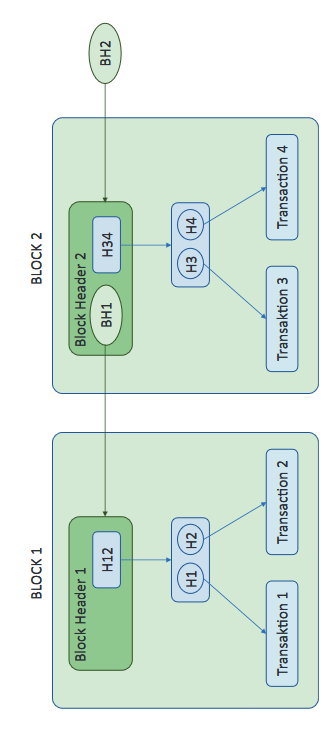
\includegraphics[width= 0.66\columnwidth]{BC_Aufbau.png}
        \quelle{\cite[p.~19]{fill2020blockchain}}
        \captionof{figure}{Aufbau einer Blockchain}
        \label{fig:BC_Aufbau}
    \end{minipage}
    \begin{minipage}{.33\textwidth}
        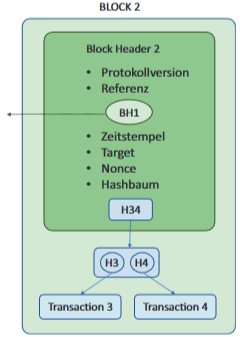
\includegraphics[width= 0.33\columnwidth]{BC_Erweiterung.png}
        \quelle{\cite[p.~24]{fill2020blockchain}}
        \caption{erweiterter Block Header für Proof-of-Work}
        \label{fig:BC_Erweiterung}
    \end{minipage}
\end{figure}


Damit ist die Blockchain ein verteiltes Register mit Integritätsgarantie. Die Integrität 
wird hierbei sichergestellt, indem eine Änderung an einem beliebigen Punkt in der
Blockchain eine Anpassung in allen Blöcken nach sich zieht, die eine direkte oder
indirekte Referenz auf diesen Block haben. Dank klarer und verschlüsselter Eigentumsansprüche
werden Änderungen nur dann vorgenommen, wenn sie berechtigt sind.
% Oder:
% Als Schutzmechanismus werden Änderungen jedoch nur dann vorgenommen, wenn sie durch 
% klare und verschlüsselte Eigentumsansprüche berechtigt sind.
\cite[p.~22]{fill2020blockchain} 

\subsubsection{Erweiterung der Blockchain mit Proof-of-Work}
\label{sec:Erweiterung}
% Erweiterung der Blockchain mittels eines Konsensalgorithmus
Neue Blöcke werden mittels eines Konsensalgorithmus hinzugefügt.
Hierfür wird zuerst ein Rechnerknoten ausgewählt, der den neuen Block berechnet. 
Da die Blockchain dezentral strukturiert ist, wird dies durch ein Zufallsprinzip entschieden.
% dezentral --> Verzicht auf Intermediäre
Hierfür wird ein kryptographisches Puzzle an alle Rechnerknoten gestellt, das ausschließlich
durch den erbrachten Rechenaufwand lösbar ist. Daher nennt sich das hier erläuterte Prinzip
"Proof-of-Work". Zuerst wird der Block Header um die für das Puzzle nötigen Elemente 
erweitert: Eine Protokollversion zum Erstellen des neuen Blocks, einen Zeitstempel mit
dem Zeitpunkt des Erstellens, einem Target als Angabe des Schwierigkeitsgrades des Puzzles
und einer Nonce (Number used once) als Beweis der Lösung des Puzzles (siehe \autoref{fig:BC_Erweiterung}).

Aus diesen erweiterten Elemente wird zusammen mit der Referenz BH1 auf den vorangehenden 
Block Header und der Wurzel H34 des Hash-Baumes auf die Transaktionsdaten ein gemeinsamer 
Hashwert berechnet. 
Das Ziel des Puzzles ist einen Hashwert zu generieren, der kleiner als das Target ist. Die 
Miner haben dafür einzig die Nonce als veränderbaren Wert zur Verfügung. Wurde das Rätsel
gelöst, wird der neue Block zusammen mit der Nonce an alle anderen Rechnerknoten zur Prüfung
geschickt.
Zuletzt wird dieser neue Block in die Blockchain aufgenommen , sofern er validiert und 
fehlerfrei ist; ansonsten wird dieser verworfen.
\cite[p.~22ff]{fill2020blockchain}


\subsection{Einsatzgebiete im Finanzsektor}
Bereits ... hat die Blockchain ihren Einzug in den Finanzsektor gefeiert. Manche
Sektoren sind aufgrund der Blockchain neu entstanden, wie der Kryptomarkt. Andere Sektoren,
wie der Aktienmarkt wurden dadurch grundlegend/stark verändert. Wieder andere Bereiche, in denen die Blockchain
einen essentiellen Teil bildet, sind nicht sehr bekannt. Im Folgenden wird der Einfluss
der Blockchain auf zuvor vorhandene Finanzsektoren, sowie neu erschlossene Sektoren 
betrachtet.

\subsubsection{Transaktionen / Kryptowährungen}
Der Kryptomarkt ist der wohl bekannteste Bereich, in der die Blockchain ein 
grundlegender Bestandteil ist. 
Die stärksten Kryptowährungen sind Bitcoin und Ethereum. 
Die Blockchain gewährleistet die Sicherheit und Nachvollziehbarkeit von Transaktionen.
\cite[p.~168]{chowdhary2025smart}
% Verweis auf vorher verifizierte Blöcke & vollst. Kopie auf jedem teilnehmenden Gerät.
So ermöglicht sie einen Peer-to-Peer Austausch von digitalen
Währungseinheiten ohne Intermediäre, wie Banken und andere Zahlungsdienstleister,
die die Vertrauenswürdigkeit der Transaktionsakteure beglaubigen sollen.
\cite[p.~32]{fill2020blockchain}
Die Nachvollziehbarkeit wird dadurch erreicht, indem die Transaktionen fest in der 
Blockchain codiert sind (siehe \autoref{fig:BC_Aufbau}).
%\cite[p.~11]{pirafelnerblockchaintechnologie}

% Sicherheit
Ein Konsensalgorithmus gewährleistet die Sicherheit und Integrität der Daten.
Am Beispiel des Bitcoin wird das Konzept \glqq Proof-of-Work\grqq{} analog zum Abschnitt 
\ref{sec:Erweiterung} angewendet. Demnach werden Änderungen von bereits getätigten
Transaktionen und neu durchgeführte Transaktionen ausschließlich in die Blockchain
aufgenommen, wenn diese von anderen Rechnerknoten validiert wurden.
% dezentral --> Verzicht auf Intermediäre
Zusätzlich ermöglicht die dezentrale Strukturierung der Blockchain den Verzicht auf 
Intermediäre, wodurch Transaktionen in einem Peer-to-Peer Netzwerk 
% also direkt von Person zu Person
durchgeführt werden können.
\cite[p.~23]{fill2020blockchain}
Dadurch sind die Kosten von Transaktionen länderunabhängig \cite[p.~12]{pirafelnerblockchaintechnologie}
und die Ausführung ist schneller 
%weniger Zwischeninstanzen durchlaufen
und kostengünstiger. \cite[p.~168]{chowdhary2025smart}


\subsubsection{Smart Contracts}
Smart Contracts sind digitalisierte und automatisierte Verträge.
\cite[p.~14]{pirafelnerblockchaintechnologie}
Treten die in ihnen definierten Bedingungen ein, so werden die einprogrammierten Aktionen
ausgeführt.
% Sie führen unter erfüllten Bedingungen die einprogrammierten Befehle, wie z.B. weitere Transaktionen aus. 
\cite[p.~55f]{fill2020blockchain}
Voraussetzung ist, dass die Blockchain-Plattform Smart Contracts in Form von 
Befehlssätzen unterstützt. Die Bitcoin-Plattform unterstützt zum Beispiel nur rudimentäre
Skripte mit denen sich hauptsächlich weitere Transaktionen automatisieren lassen. 
Außerdem sind die verfügbaren Befehle in keinem Dokument spezifiziert und sind nur auf
der Code-Basis der Plattform einsehbar.
Im Gegensatz dazu stellt die Ethereum-Plattform einen viel umfangreicheren Befehlssatz
zur Verfügung. Dieser ist sogar Turing-Vollständig, was ihn dieselbe Mächtigkeit wie
herkömmliche Programmiersprache haben lässt. 

Ebenso wie verschiedene Programmiersprachen den Befehlssatz eines Rechners umsetzen
%Googlen!!!
existieren mehrere Programmiersprachen, die den Befehlssatz für Smart Contracts
syntaktisch leichter nutzbar machen. Die bekannteste für Ethereum ist hier Solidity,
die 2014 von Dr. Gavin Wood vorgestellt wurde. Da die Ausführung eines Smart Contracts
in den einzelnen Rechnerknoten, also bei den Minern, stattfindet, ist es unerlässlich, 
dass die verwendete Sprache auf jeder Rechnerarchitektur interpretiert werden kann.
% Die wichtigste Eigenschaft für jede Programmiersprache um Smart Contracts zu definieren ist, dass sie auf jeder Rechnerarchitektur, unabhängig von der Hard-Ware und dem verwendeten Prozessor, funktioniert. 
Dazu wird der Code des Smart Contract vom Compiler in 
Bytecode umgewandelt und als dieser durch eine Transaktion in die Blockchain 
aufgenommen. % eingefügt
%Ausführung eines SC
Sobald ein Smart Contract von einer Transaktion aufgerufen wird, wird der Bytecode 
auf der Ethereum Virtual Machine interpretiert.
Sobald ein Smart Contract von einer anderen Transaktion aufgerufen wird, hat sie 
Zugriff auf einige Daten innerhalb der BlockChain. Ihr liegen sämtliche Informationen
in ihrem

\cite[p.~57ff]{fill2020blockchain}





\subsubsection{Tokenization von Assets}

% \subsubsection{Smart Grid im Energiesektor}
% Besser im Kapitel Nachhaltigkeit!
% \cite[p.~72]{fill2020blockchain}


\subsection{Risiken bei der Integration von Blockshains}
\cite[p.~17]{pirafelnerblockchaintechnologie}